\documentclass[a4paper, 14pt]{extarticle}
\usepackage[utf8]{inputenc}
\usepackage[russian]{babel}
\usepackage{amsmath}
\usepackage{amsfonts}
\usepackage{amssymb}
\usepackage{caption}
\usepackage{subcaption}
\usepackage{graphicx}
\usepackage{textcomp}
\usepackage{placeins}
\setcounter{page}{46}
\begin{document}
\section*{Приложение}
\subsection*{Приложение 1}
\begin{figure}[!h]
	\centering
	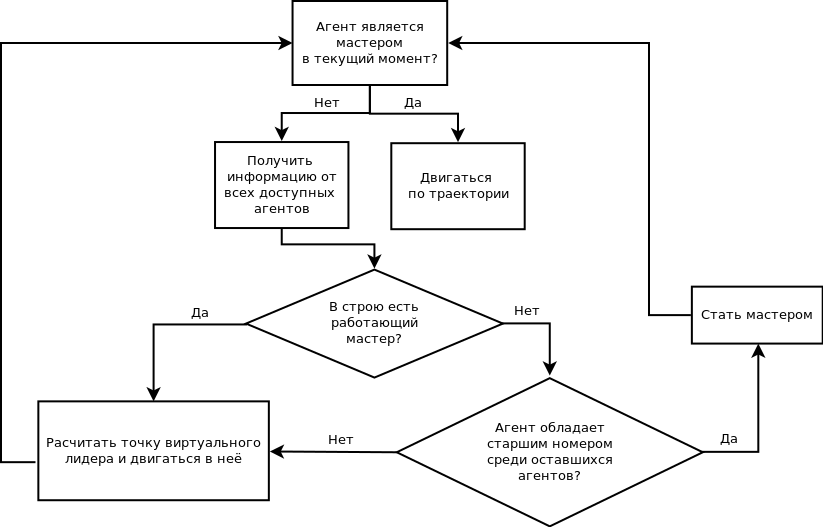
\includegraphics[width=1\linewidth]{others/algo-dia}
	\caption{Блок-схема алгоритма управления, который выполняет каждый агент}
	\label{fig:algo-dia}
\end{figure}
\subsection*{Приложение 2}
Исходный код реализованного алгоритма можно найти в git репозитории https://github.com/xozzslip/agents-platooning. 
\end{document}

